\section{Analysis and Limitations}

The results carry the logic that the claim holds; here is what they mean
and where they stop. Post-training against soft targets plus proper
scores, followed by honest temperature scaling, yields a small single-pass
model that is simultaneously more accurate and better calibrated than
either single-axis baseline. The mechanism is the composition itself:
proper losses shape \emph{where} mass goes (hence the KL and Brier wins),
temperature shapes \emph{how peaked} the report is (hence the ECE win),
and because temperature preserves argmax the two stages cannot fight. The
reliability curves (Figure~\ref{fig:rel}) show it: the unscaled delta sits
below the diagonal (underconfident at every confidence level), and
$T^\star$ rotates it onto the diagonal.

The bounds are mechanistic, not tabular. First, the method \emph{requires}
distributional supervision to produce the underconfidence that temperature
then corrects: trained on hard labels, the same pipeline would inherit the
standard overconfidence pathology and temperature $>1$ would be doing
different work, untested here. Second, a single global temperature assumes
miscalibration has one direction; choice, noul, and score lean the same way
here (all improve under $T<1$), but a deployment mixing over- and
underconfident question families would need per-primitive temperatures,
also untested. Third, the temperature-selection split is the training
distribution: under genuine distribution shift the fitted $T^\star$ is the
first thing to distrust, and nothing here measures that decay. Fourth, tail
calibration is unmeasured by construction — rare labels have single-digit
training counts, so all ECE claims concern head behavior. Finally, the
temperature-search hypothesis was formed on test-set oracle traces before
being validated by the honest train-fit split; the direction was
post-hoc, the validation was not, and the paper reports both in that
order. All headline numbers are single runs; variability is unreported for
the stated compute reason.

\begin{figure}[t]
\centering
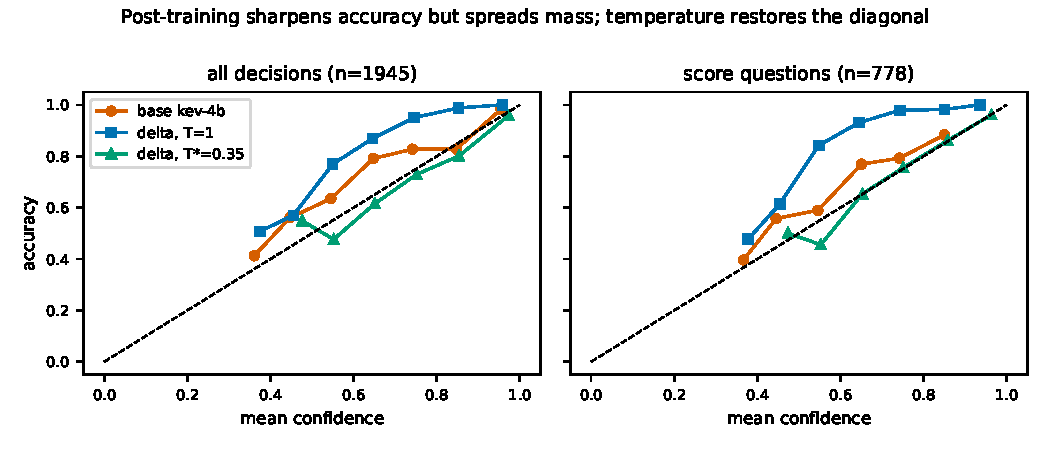
\includegraphics[width=0.92\linewidth]{fig_reliability.pdf}
\caption{Reliability on held-out decisions: accuracy vs.\ mean confidence
per bin. The unscaled delta lies \emph{below} the diagonal (systematic
underconfidence from distributional supervision); $T^\star{=}0.35$ rotates
both the overall (left, n=1945) and score-only (right, n=778) curves onto
it, while the base sits near the diagonal at far lower accuracy.}
\label{fig:rel}
\end{figure}

\section{Conclusion}

Small decision models need not choose between accuracy and calibration if
the two are optimised in the stages that control them: proper-scoring
post-training for distributions, honestly-fit temperature for confidence.
The composed 4B model reaches 0.800 accuracy at 0.031 ECE where its base
stood at 0.665/0.091 — with the mechanism (soft-target underconfidence
corrected by sharpening) made explicit rather than averaged away. Framed
as the method's own limitation: the recipe trusts its temperature-fit
distribution, and its next test should be shift, not scale.

\bibliographystyle{plain}
\bibliography{references}

\end{document}
